\documentclass[12pt]{standalone}

\usepackage{tikz}

\begin{document}
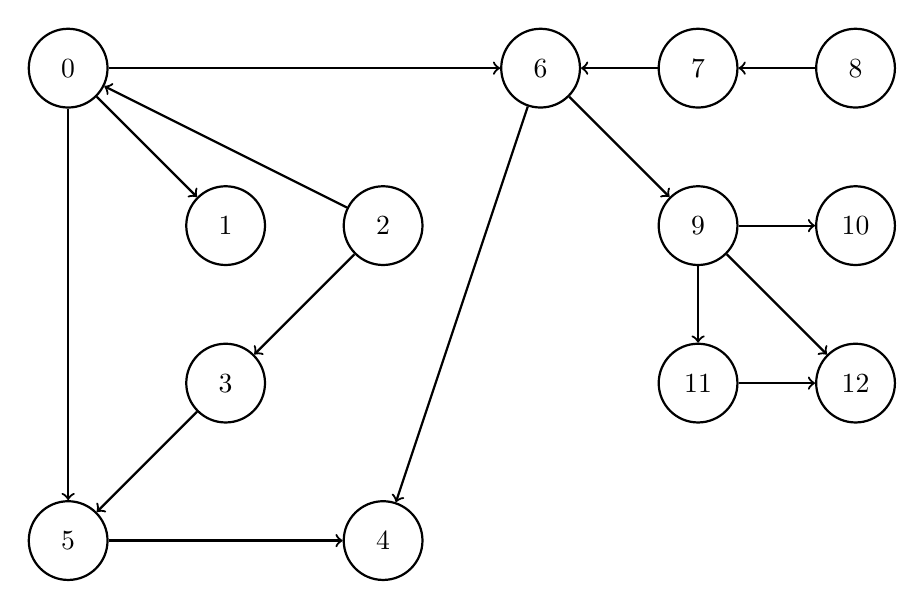
\begin{tikzpicture}[x=2cm,y=2cm,thick]
    \begin{scope}[every node/.style={circle,draw,minimum size=1cm}]
        \node (0) at (0,3) {0};
        \node (1) at (1,2) {1};
        \node (2) at (2,2) {2};
        \node (3) at (1,1) {3};
        \node (4) at (2,0) {4};
        \node (5) at (0,0) {5};
        \node (6) at (3,3) {6};
        \node (7) at (4,3) {7};
        \node (8) at (5,3) {8};
        \node (9) at (4,2) {9};
        \node (10) at (5,2) {10};
        \node (11) at (4,1) {11};
        \node (12) at (5,1) {12};
    \end{scope}

    \path[->]
        (0) edge (1) edge (5) edge (6)
        (2) edge (0) edge (3)
        (3) edge (5)
        (5) edge (4)
        (6) edge (4) edge (9)
        (7) edge (6)
        (8) edge (7)
        (9) edge (10) edge (11) edge (12)
        (11) edge (12);
\end{tikzpicture}
\end{document}
